\documentclass[aps,pre,twocolumn,showpacs,showkeys]{revtex4-1}
 %\pdfoutput=1 \input epsf

\usepackage[utf8]{inputenc}
\usepackage[english]{babel}
\usepackage{hyperref}

\usepackage{amsmath}
\usepackage{amssymb}
\usepackage{amscd}
\usepackage{mathtools}

\usepackage{color}
\usepackage{graphicx}
\usepackage{subfigure}

\usepackage{upgreek}
\usepackage{dcolumn}
\usepackage{natbib}

\DeclareMathOperator{\erfc}{erfc}

\newcommand{\rmd}{{\mathrm d}}
\newcommand{\rme}{{\mathrm e}}

\renewcommand{\vec}[1]{{\boldsymbol {#1}}}
 %  \usepackage{showkeys}

\begin{document} 

\title{The interaction between Actin and Myosin-II, the flashing ratchet}
\author{Pieter Baerts}
\author{Christian Maes}
\affiliation{KU Leuven, Instituut voor Theoretishe Fysica, Celestijnenlaan 200D, B-3001 Leuven, Belgium}
\author{Jiří Pešek}
\author{Herman Ramon}
\affiliation{KU Leuven, BIOSYST-MeBioS, Kasteelpark Arenberg 30, B-3001 Leuven, Belgium}

\begin{abstract}
We present a model for the movement of a myosin-II molecular motor along a straight actin filament, in which the heads of the motor are subjected to a flashing ratchet potential. This simple model already features the force-velocity relation and aspects of mechanosensing. We also investigate the energy input from the chemical ATP cycle and its dependence on external loads on the motor.  
\end{abstract}

\maketitle 

\section{Introduction}

The cytoskeleton of a cell serves two main purposes, being transporting large vesicles and governing the cell's motility, i.e. the ability of the cell to move and change its shape. 
It mainly consists of long semi-flexible polymers and molecular motors. 
These motors contain several heads that are able to bind to polymer filaments and walk along them. 
The mechanism for walking relies both on a chemical cycle in the motor's head and on the asymmetry of a periodic and electrostatic potential along the length of such a polymer.


The chemical cycle is driven by ATP molecules that can attach to a motor head, causing it to change the charge of the head and consequently loosen its bond with the polymer filament. 
When bound to a motor head, the ATP molecule will hydrolyze to ADP and release a phosphate. 
It this state, the head can attach to the polymer again, ADP will be released from the motor head and the chemical cycle can start over. 
Hence, the chemical state of a motor head will determine how strongly it can be coupled to a cytoskeletal filament. 


Cytoskeletal polymers exhibit a sequence of monomers that cause a periodical structure. 
Furthermore, these monomers are polarised, so that when chained together in a polymer, they give rise to a symmetric, ratchet-like, electrostatic potential along the length of the filament. 
An example of such a potential is shown in figure \ref{Fig: ratchet setup}. 
The heads of a motor, too, carry an electric charge and therefore they will feel the ratchet potential of the filaments. 
In the attached state, the motor will tend to be close to minimal potential energy. 
However, when the chemical state of the head changes, so does its molecular structure and charge. 
As mentioned earlier, this causes the bond between the head and a filament to either strengthen or loosen. 
Therefore the head will experience a ratchet potential that is flashing in time, changing the amplitude of the potential from high to low.


When tightly bound, the head will most probably be very close to a minimum in the ratchet potential, while in the unbound state, it is easier for the motor to diffuse over a larger distance. 
However, because of the asymmetry of the ratchet, the motor will be biased to explore one side of the ratchet rather than the other. 
Therefore, the motor will more likely jump to an adjacent period of the ratchet potential in the preferred direction, indicated by the asymmetry of the potential. 
This will eventually lead to ballistic motion of the motor on long timescales.


The part of the cytoskeleton that is mainly responsible for the motility of the cell is the actin-myosin cortex and it will serve as the exemplary system in this paper.


Ratchet models have been studied extensively in the context of molecular motors REFF(astumian, jullicher, Huxley, Hanggi,...). %TODO
The models that have been used in these studies are very similar to each other but ofter differ in some basic assumptions.
The specific model that we have studied is presented in section \ref{sec:ratchet} and has following important traits:
\begin{itemize}
\item The chemical rates do not depend on spacial degrees of freedom. 
Motor heads can attach and detach anywhere along the polymer filament.
\item The chemical rates are independent of external forces on the motor.
\item The motors are rigid with equal spacing between the heads.
\end{itemize} 
Furthermore we will be studying non-muscle myosin II motors, that have a small number of heads. 
These motors are believed to be crucial the motility in eukaryotic cells.
For larger myosin motors, like the ones in muscle cells, mean-field calculations have lead to analytic results for the force-velocity relation REFF(Jullicher). %TODO
In experimental studies with synthetic myosin motors, the number of heads per motor is also much higher than in non-muscle cells. 
Therefore, the results for large motor play a very important role in interpreting and understanding those in-vitro experiments REFF. %TODO
For motors with fewer heads, mean-field methods are not suitable and numerical simulations prove to be useful.
In section III. we will describe the movement of this motor-polymer system in detail by means of computational simulations. %XXX


Another important aspect of molecular motors is their ability to convert chemical energy into mechanical work REFF. %TODO
The chemical cycle of ATP hydrolysis consists out of many consecutive reactions and after one full cycle a net amount of energy is provided to the motor head REFF. %TODO
However, often this cycle is represented by only two states, e.g. ATP bound and ADP bound, 
in which case a stochastic process on these states always satisfies detailed balance and no chemical energy can be extracted. 
In other words, the gain of one reaction is canceled by the cost of the following reaction.
On the other hand we do not want any redundant degrees of freedom in our description since we are not really interested in the full chemical details of the process.
In section IV, we will look at an alternative way of interpreting the chemical input by measuring the differences in potential energy in each jump and we define a chemical efficiency. %XXX
In section V. we provide a perturbative calculation to validate and understand some features of this chemical efficiency and how it changes when the motor is under external load. %XXX


Lastly, in section VI., we look at the coupling of the motor to an elastic environment. %XXX
Earlier studies have shown that  motors are able to sense the stiffness of their environment and that they can adapt the active forces that they generate REFF. %TODO
In those studies the rates did depend on the load on the motor. We show computationally that a motor in our simple ratchet model with constant rates behaves similarly.


\section{The Ratchet model}
\label{sec:ratchet}
In order to investage the movement of myosin along the actin filament we consider the following one dimensional model:
First, we assume that the rigidity of the actin polymer and myosin backbone is high enough that their elongations can be neglected.
Second, we assume that all myosin heads are attached directly to the myosin backbone at fixed equidistant positions, see figure~\ref{Fig: ratchet setup}. 
These simplifications allow us to model both, the motor and the filament, as point particles undergoing overdamped diffusion \cite{}. %TODO
Moreover, each myosin head has an internal state, which represent its chemical state, 
i.e. whether there is an ATP bounded or not to the myosin head. 

The dynamics of the full system is then described by coupled overdamped Langevin equations 
\begin{align}
&\begin{multlined}[b]
\rmd x_\text{M} = 
\frac{1}{\gamma_\text{M}} \left[ - \nabla_\text{M} V_t(x_\text{M}(t) - x_\text{A}(t)) + F_\text{load} \right] \; \rmd t 
\\ 
+ \sqrt{ \frac{2 k_B T}{\gamma_\text{M}} } \; \rmd W_\text{M} ,
\end{multlined}
\label{eom_M} \\
&\begin{multlined}[b][.42\textwidth]
\rmd x_\text{A} = 
- \frac{1}{\gamma_\text{A}} \nabla_\text{A} V_t(x_\text{M}(t) - x_\text{A}(t)) \; \rmd t 
\\
+ \sqrt{ \frac{2 k_B T}{\gamma_\text{A}} } \; \rmd W_\text{A} ,
\end{multlined}
\label{eom_A}
\end{align}
where $x_\text{M}$ ($x_\text{A}$) denote the position of myosin (actin polymer), 
$\gamma$ is the Stokes drag,
$T$ is the absolute temperature of the environment,
$W$ denotes the Wiener process,
$F_\text{load}$ is an external load on the motor, 
and the interaction potential $V_t$ represents the overall ratchet interaction, which is a sum over individual contributions from all motor heads,
\begin{equation}
V_t(x) = \sum\limits_{i=0}^{N-1} \zeta_t(i) \, V_\text{r} (x - i \, d ), 
\end{equation}
where $d$ is the distance between myosin heads, 
$N$ is the number of heads per motor,
$\zeta_t(i)$ represents the internal state, see bellow, 
and $V_\text{r}$ is the periodical ratchet potential, see figure~\ref{}, %TODO 
\begin{equation}
V_\text{r}(x) =  \begin{cases}
        V_\text{r}(x+\ell) & x < 0 \\[1ex] 
        \displaystyle \frac{ V x }{ a \ell } & 0 \leq x < a \ell \\[2ex]
        \displaystyle \frac{ V (\ell-x) }{ (1-a) \ell } & a \ell \leq x < \ell \\[2ex]
        V_\text{r}(x-\ell) & \ell \leq x  
   \end{cases} ,
   \label{rat_pot}
\end{equation}
with total height $V$,
period $\ell$ 
and skewness parameter $a \in [0,1]$. 

%%%%%%%%%%%%%%%%%%%
Unlike in traditional models \cite{}, %TODO
in our model the internal state represents whether ATP is bound or unbound to the myosin head. 
This change, of motor heads evolve as a continuous time Markov jump process with rates $k_\text{bind}$, $k_\text{unbind}$ 
\begin{equation}
\zeta_t = 1 \overset{k_\text{bind}}{\underset{k_\text{unbind}}{\rightleftarrows}} \zeta_t = c
\end{equation}
where $c\in\left[0,1\right]$. 
The parameter $c$ determines the amplitude of the ratchet potential when the motor is loosely bound to the filament. 
The evolution of the internal state of the heads, i.e. a two-level system, is governed by the rate for going from state $0$ to $1$ is $k_{a}$ and the reverse rate is $k_{d}$.
These rates depend on the concentrations of the relevant chemical species present in ATP hydrolysis, more specifically $k_{d}$ is proportional to $[\text{ATP}]$ while $k_{a}$ is proportional to the inverse of $[\text{ADP}]$ and $[\text{P}_\text{i}]$ [REF]. 
Figure \ref{Fig: ratchet setup} depicts the whole setup of motor and flashing ratchet. 
\begin{figure}[t]
\centering
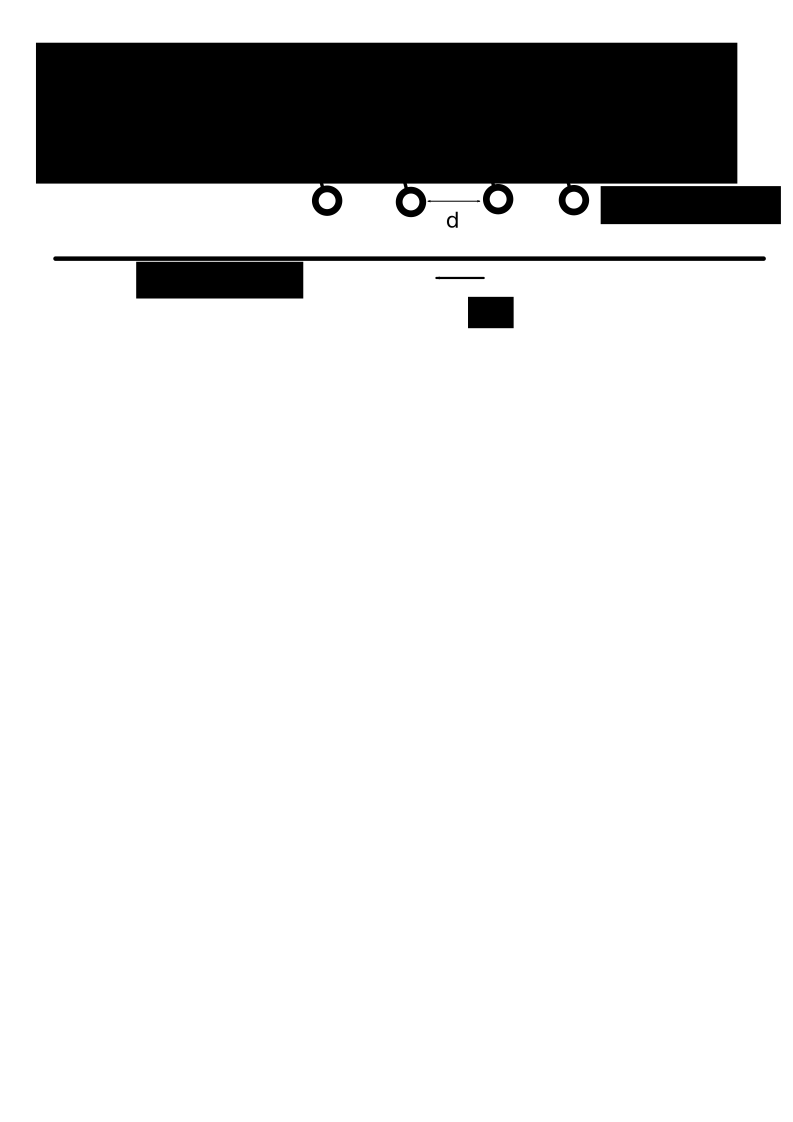
\includegraphics[width=0.45\textwidth,height=!]{ratchet_illustration}
\caption{In the top of this illustration, the backbone of the myosin motor is shown with heads that are a distance $l$ apart. 
In the bottom, the potential along an actin filament is depicted. 
It had a period $d$ and skewness $a$. 
Depending on the internal state of the motor head, it will feel a ratchet potential with hight $V$ or $cV$.} 
\label{Fig: ratchet setup}
\end{figure}

Table \ref{Tab: Parameters} lists the values of the parameters used in this model. 
Some of them were took from the literature while others were fitted to give a realistic speeds and stall force for the myosin II motor. 
The friction coefficients were calculated with Stokes' law, using the known dimensions of the molecules \footnote{The myosin II motor and actin filament molecules were approximated in this calculation by long, thin cylinders.} and the viscosity of the extracellular medium.
\begin{table}[t]
\centering
\begin{tabular}{lcdcc}
Parameter & Symbol & \multicolumn{1}{c}{Value} & Units & Source\\
\hline\hline
Thermal energy& $k_B T$ & 4.28 & pN nm & --- \\
Number of heads& $N$ & 4 & --- & REF\\
Head's spacing& $l$ & 15 & nm & REF\\
Step length& $d$ & 8 & nm & REF\\
Binding rate& $k_{a}$ & 40 & s$^{-1}$ & REF\\
Detaching rate& $k_{d}$ & 80 & s$^{-1}$ & REF\\
Skewness& $a$ & 0.25 & --- & ---\\
Potential amplitude& $V$ & 40 & pN nm & ---\\
Potential scaling& $c$ & 0.3 & --- & ---\\
Motor friction& $\gamma_{m}$ & 0.66 & pN $\upmu$s nm$^{-1}$ & REF\\
Actin friction& $\gamma_{a}$ & 0.97 & pN $\upmu$s nm$^{-1}$ & REF\\
\end{tabular}
\caption{Table of all parameter values and a reference to their source.}
\label{Tab: Parameters}
\end{table}

While both the diffusion and the jump process are in equilibrium, the mechanism of the flashing ratchet brings the combined system out of equilibrium, leading to the movement of the motor in a preferred direction, given by the asymmetry of the filament. 
In simulations we measured the mean velocity $\langle v\rangle$ of the motor with respect to the filament. 
This for different values of $c$, the scaling factor of the amplitude of the ratchet potential, show in figure \ref{Fig: c_v}.
\begin{figure}[t]
\centering
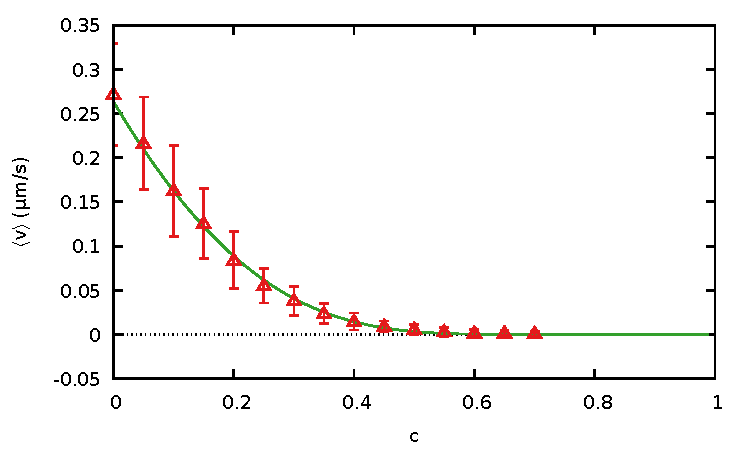
\includegraphics[width=0.45\textwidth,height=!]{c_v_4heads}
\caption{Mean velocity $\langle v \rangle$ of the motor relative to the actin filament for $c \in (0,1)$.
The mean velocity rapidly decreases towards the $0$ as we approach equilibrium, $c \to 1$.  
Green line correspond to the fit $ \left\langle v \right\rangle \propto \exp ( - \frac{\alpha}{1-c} ) $.
%The dependency is guessed, unfortunately I don't have any argument to support it. 
} 
\label{Fig: c_v}
\end{figure}
We see that mean velocity goes to zero when $c$ approaches $1$. 
This is to be expected since $c=1$ corresponds to the case where there is no more flashing of the potential, hence the system is in equilibrium.


Alternatively, the mean velocity also depends on the concentration of ATP through the detach rate $k_{d}$. 
This dependency is show in figure \ref{Fig: v_k}.
\begin{figure}[t]
\centering
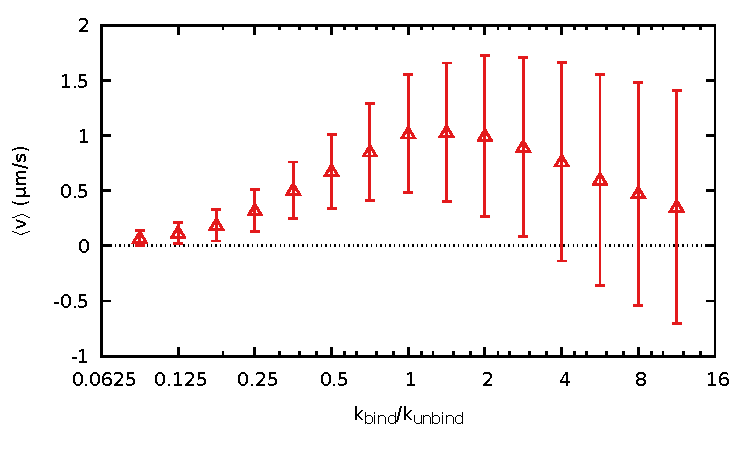
\includegraphics[width=0.45\textwidth,height=!]{v_k}
\caption{Mean velocity of the motor relative to the actin filament $\langle v \rangle$ for varying $k_{d}$.
The velocity decreases to $0$ for large discrepancies between attach and detach rates and reaches when they are comparable.
}
\label{Fig: v_k} 
\end{figure}
The first data point corresponds to the case where $k_{d} = k_{a} = 40 s^{-1}$ and for the following points $k_{d}$ is doubled every time while $k_{a}$ stays constant. 
We first observe that the velocity initially increases, then reaches a maximum around $k_{d} = 160 s^{-1}$ and finally decreases again. 
A high detach rate means that the motor heads will be attached only for a short time. 
If this time is too short, the motor might not diffuse all the way to the minimum of the ratchet and has a higher probability the move against the direction given by the asymmetry of the potential. 
On the other hand, when the detach rate is low the motor has a lot of time to fully equilibrate and will no longer contribute to the generated current. 
The simulations show that there is an optimal value of$k_{d}$ to maximize the relative velocity between the motor and the actin filament. 



\section{Force-velocity relation}
In this section, an external load force $F_\text{load}$ is applied to the motor, as in equation (\ref{eom_M}). 
When applying a force against the preferred direction of the motor, it is expected to slow down. 
The force that is needed to stop the motor, relative to the actin filament, is called the stall force, i.e. 
\[
\left\langle v ( F_{load} = -F_{stall} ) \right\rangle = 0 .
\]
Figure \ref{Fig: F_v_zoom}  shows the results from simulations of the motor under load. 
The intersections of the curves with the vertical axis correspond to the mean velocities in figure \ref{Fig: v_k} . 
We see that the mean velocity decreases linearly with increasing load. 
The slope varies for different detach rates. This can be understood by observing the dependency of the stall force on $k_{d}$ in figure \ref{Fig: k_Fstall}.
\begin{figure}[t]
\centering
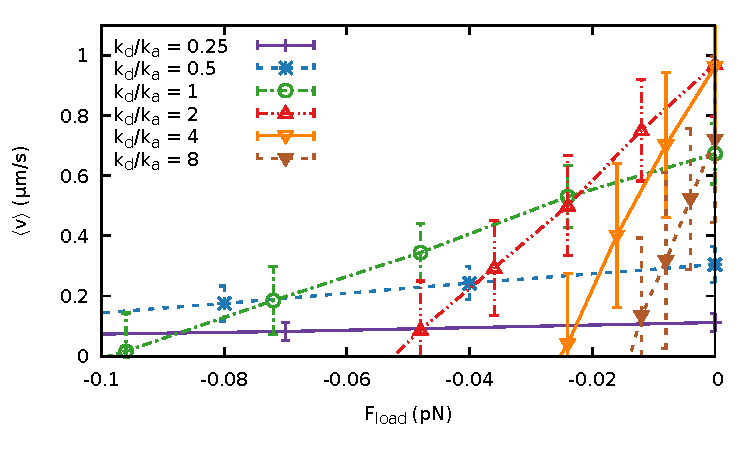
\includegraphics[width=0.45\textwidth,height=!]{F_v_zoom}
\caption{Mean velocity of the motor $\langle v \rangle$ with a small load force $F_\text{load}$ applied in the direction opposing the movement for different detach rates $k_d$.
Intersections with the $x$ axis correspond to stall forces for given detach rates. 
We can see that with increasing $k_d/k_a$ ratio the slope increases as well as the full curve shifts in the low force region, causing a persistent decrease in stall force.  
}
\label{Fig: F_v_zoom} 
\end{figure}

\begin{figure}[t]
\centering
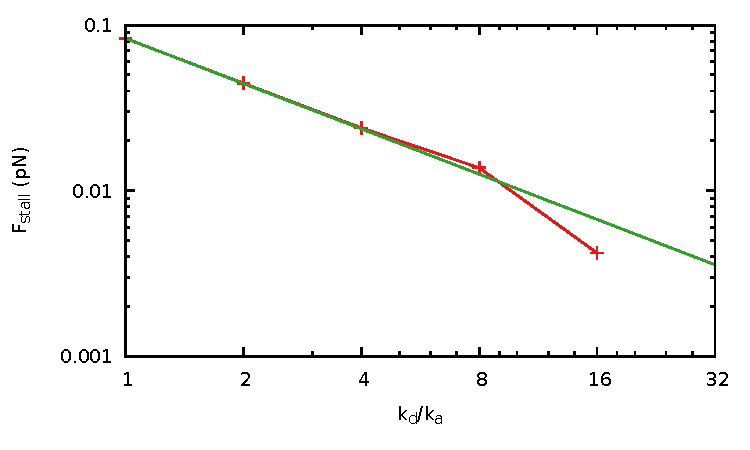
\includegraphics[width=0.45\textwidth,height=!]{k_Fstall}
\caption{Stall force $F_\text{stall}$ for different detach rates $k_\text{d}$.
We observe power-law decay $F_\text{stall} \propto k_\text{d}^{-\alpha}$ with exponent $\alpha = 1.002 \pm 0.014$. 
}
\label{Fig: k_Fstall} 
\end{figure}
When the detach rate $k_{d}$ increases, so does the fraction of time in which the motor is the least bound to the actin filament. 
Hence, it will take a smaller load to halt a motor since the amplitude of its confining potential will be lower on average.
In figure \ref{Fig: F_v} the mean velocity of the motor with respect to the actin filament is plotted for a wider range of the load force. 
As a reference, the speed of a non-interacting motor, i.e. $\langle v \rangle = \frac{1}{\gamma_M}F_{load}$, is shown in black as a reference.
\begin{figure}[t]
\centering
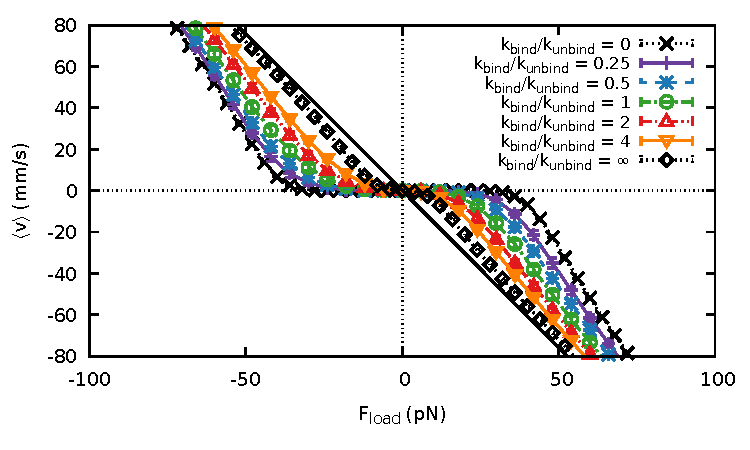
\includegraphics[width=0.45\textwidth,height=!]{F_v}
\caption{Mean velocity $\langle v \rangle$ of the motor as a function of the load force $F_\text{load}$ for $c=0.3$ and $k_d/k_a = 2$.}
\label{Fig: F_v} 
\end{figure}
For small load forces, there is a regime in which the response is very low. 
The ratchet interaction provides a friction force to counter the load force. 
For larger forces the system looses its resilience and the contribution from the load will dominate. 
The larger the load, the more the velocity will approach  $\frac{1}{\gamma_M}F_{load}$.
Curves for higher detach rates are closer to the curve for the completely unbound motor. 
The motor is more submissive to the external load, which can be understood through the same reasoning as for the stall force.
It is also interesting to investigate the velocities of the motor and actin filament with respect to an inertial frame of reference, instead of the relative velocity to each other. 
For equations (\ref{eom_M}) and (\ref{eom_A}) we can obtain the following.

\begin{align*}
\gamma_M \langle v_M \rangle &= \langle F_r \rangle + F_{load} \\
\gamma_A \langle v_A \rangle &= -\langle F_r \rangle
\end{align*}
Where $\langle v_{M,A} \rangle = \langle \frac{\rmd x_{M,A}}{\rmd t} \rangle$ 
and $\langle F_r \rangle = - \langle \nabla_M V_t(x_M - x_A ) \rangle = \langle \nabla_A V_t(x_M - x_A ) \rangle $. 
And since the relative velocity is $\langle v \rangle = \langle v_{M} \rangle - \langle v_{A} \rangle$ we get
\begin{equation*}
\langle v \rangle = \frac{\gamma_A + \gamma_M}{\gamma_A \gamma_M} \langle F_r \rangle + \frac{1}{\gamma_M} F_{load}
\end{equation*}
or similarly
\begin{align}
\langle v_M \rangle &= \frac{1}{ \gamma_A + \gamma_M } \left( \gamma_A \langle v \rangle + F_{load} \right) \label{velocity_M} \\
\langle v_A \rangle &= -\frac{1}{ \gamma_A + \gamma_M } \left( \gamma_M \langle v \rangle - F_{load} \right)
\label{velocity_A}
\end{align}

\begin{figure}[t]
\centering
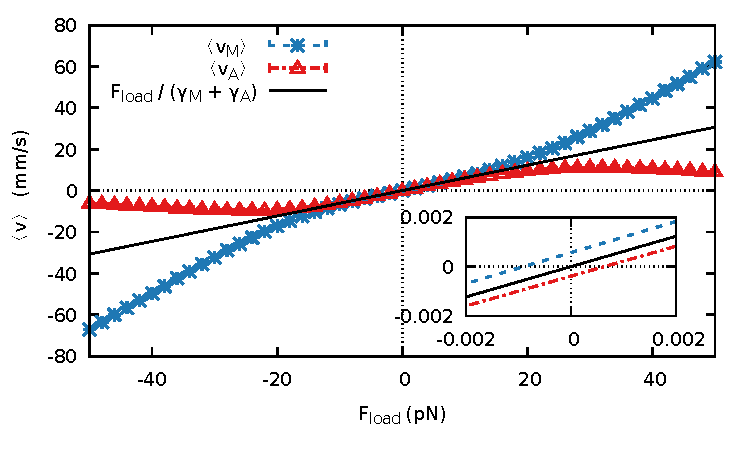
\includegraphics[width=0.45\textwidth,height=!]{individual_velocities}
\caption{Mean velocities of the motor and actin filament with respect to an inertial frame of reference for $k_d/k_a = 2$.
We observe that only the myosin is moving while the velocity of the dragged actin filament decreases as we increase the load on the myosin motor.
Inset: Zoomed to the linear regime around the origin.
}
\label{Fig: ind_v} 
\end{figure}
For figure \ref{Fig: ind_v} we can observe that already for small loads, the motor and actin filament start moving together, i.e. they are coupled by the ratchet interaction. 
In the inset of figure \ref{Fig: ind_v} their velocities, for small loads, go like $F_{load}/(\gamma_M + \gamma_A)$. 
This can be derived from equations (\ref{velocity_M}) and (\ref{velocity_A}) and the fact that the relative velocity $\langle v \rangle$ remains almost constant around the origin in figure \ref{Fig: F_v}. 
Note that at the point where the velocity of the motor drops beneath actin's velocity, the load is equal to the stall force.
Since the load is only applied to the motor, for very high loads, the motor will start slipping over the ratchet potential along the actin filament. 
Consequently, the filament's velocity will stop increase and approaches zero for larger loads. 
The motor will accelerate for higher loads and its velocity will go to $F_{load}/\gamma_M$. 
The relative velocity $\langle v \rangle$ will be equal to the motor's velocity $\langle v_M \rangle$ in that case.

Alternatively one could look at the nonlinear force-velocity relation by identifying an effective friction force that depends on the load. 
Without the ratchet interaction, the motion of the motor would satisfy following equation for the mean velocity, e.g. the black curve in figure \ref{Fig: F_v}.
\begin{equation*}
\gamma_{m}\langle v\rangle - F_{load} = 0
\end{equation*}
The violation of this relation in the presence of the ratchet interaction gives us this effective force. 
It is shown in figure \ref{Fig: effective_force}. 
Note that this is the same as the distance between the force-velocity curves and the ratchet-free curve in figure \ref{Fig: F_v}.
\begin{equation*}
\gamma_{m} \langle v \rangle - F_{load} = \frac{\gamma_A + \gamma_M}{\gamma_A} \langle F_r \rangle = F_{eff}
\end{equation*}
\begin{figure}[t]
\centering
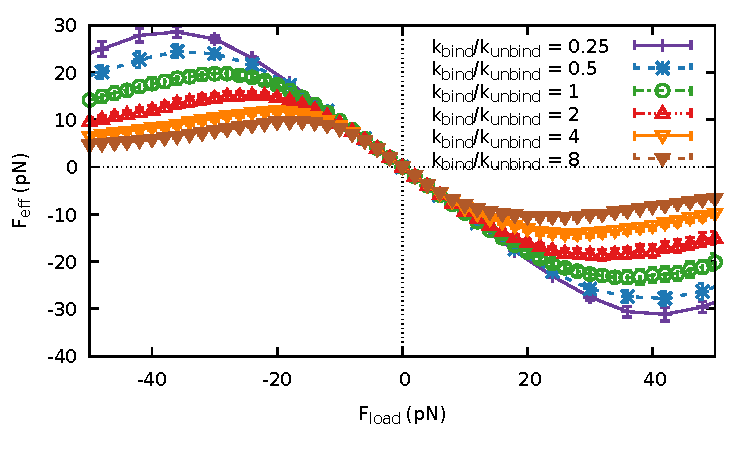
\includegraphics[width=0.45\textwidth,height=!]{effective_friction}
\caption{Effective force from the ratchet interaction depending on the load force on the motor.}
\label{Fig: effective_force}
\end{figure}
The response of the system for small loads is linear and independent of the ATP concentration. 
The effective force generated by the ratchet interaction will reach a maximal value and eventually decay for larger external forces. 
As the load goes to infinity, the friction provided by the ratchet will go to zero as 
\begin{equation}
\left| \langle F_\text{eff} \rangle_{F_\text{load}\rightarrow\infty} \right| \asymp \frac{1}{F_\text{load}} , 
\label{eq:eff_vs_load}
\end{equation} 
which is shown in figure \ref{Fig: eff_frict_decay}. 
Later on, we will show that for a one headed motor, this is indeed the dominant contribution for large external forces.  
\begin{figure}[t]
\centering
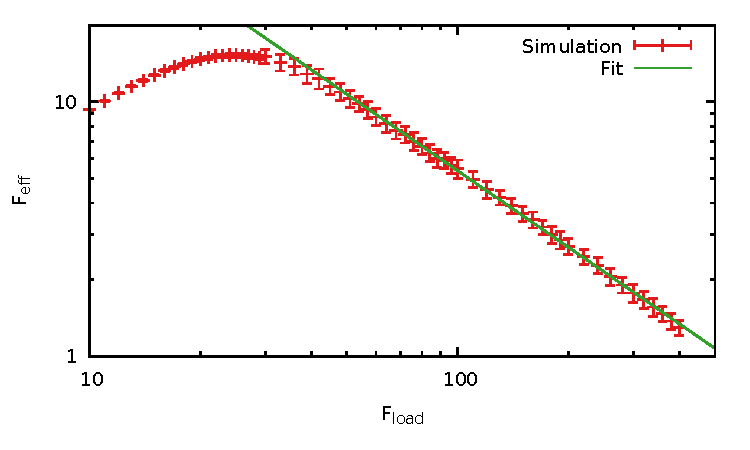
\includegraphics[width=0.45\textwidth,height=!]{eff_frict_decay}
\caption{The effective force, depending on the load, is shown in a logarithmic plot. 
We can see, that the effective friction asymptotically decay according to the power law $F_\text{eff} \propto F_\text{load}^{-\alpha}$, 
with exponent determined from the fit to be $\alpha = 0.9990 \pm 0.0047$, 
which is in good agreement with the theoretical prediction \eqref{eq:eff_vs_load}.
}
\label{Fig: eff_frict_decay}
\end{figure}


\section{Energy input from the chemical process}

The chemical cycle of the motor heads, driven by ATP, is modeled by a two-state continuous time jump process. 
The dynamics of the system is fully determined by the two rates $k_a$ and $k_d$. 
The evolution of probability density of the system $\rho_s$ is governed by the master equation, where $s = \{0,1\}$ is the chemical state of a motor head. 
State $s=0$ corresponds to an ATP bound head, loosely bound to the actin filament, while in the state $s=1$ the head is strongly coupled to the ratchet potential along the actin filament.
\begin{align*}
\dot{\rho}_0 &= -k_a \rho_0 + k_d \rho_1 \\
\dot{\rho}_1 &= k_a \rho_0 - k_d \rho_1 
\end{align*}
This system will always relax to its equilibrium steady state $\rho^{eq}_s$.
\begin{align*}
\rho^{eq}_0 &= \frac{k_d}{k_a+k_d}\\
\rho^{eq}_1 &= \frac{k_a}{k_a+k_d} 
\end{align*}
In equilibrium, detailed balance is satisfied and the chemical cycle does not dissipate heat on its own, on average.
Similarly, the diffusion processes of the myosin and actin own their own, without an external force, are in equilibrium.
However, when coupled together, we observe the motor walking along the actin track. 
This suggests that non-equilibrium is caused be the relaxation of the diffusion processes immediately after each change in the chemical state of a motor head. 
The energy that is dissipated in these recurring relaxations is provided by the changes in potential energy during each chemical jump. 
Figure \ref{Fig: energy} shows the energy landscape in which the myosin motor diffuses, relative to the actin filament. 
In state $s=0$ the motor head moves in the top ratchet, at a higher energy but with a smaller amplitude, while in state $s=1$ the head's coupling is stronger and the amplitude of the ratchet is higher. 
To each jump there is an amount of energy that is absorbed or dissipated by the system. 
We can count all the contributions of jumps to state $s=1$ and to state $s=0$ separately.
\begin{align}
\mathcal Q_{in} &= \sum_{t_d} \left[ \Delta E + (c-1) V_r(x_{t_d}) \right]  \label{q_in} \\
\mathcal Q_{out} &= -\sum_{t_a} \left[ \Delta E + (c-1) V_r(x_{t_a}) \right]  \label{q_out}
\end{align}
Where $t_a$ and $t_d$ are all jump times to state $s=1$ and $s=0$ respectively. 
\begin{figure}[t]
\centering
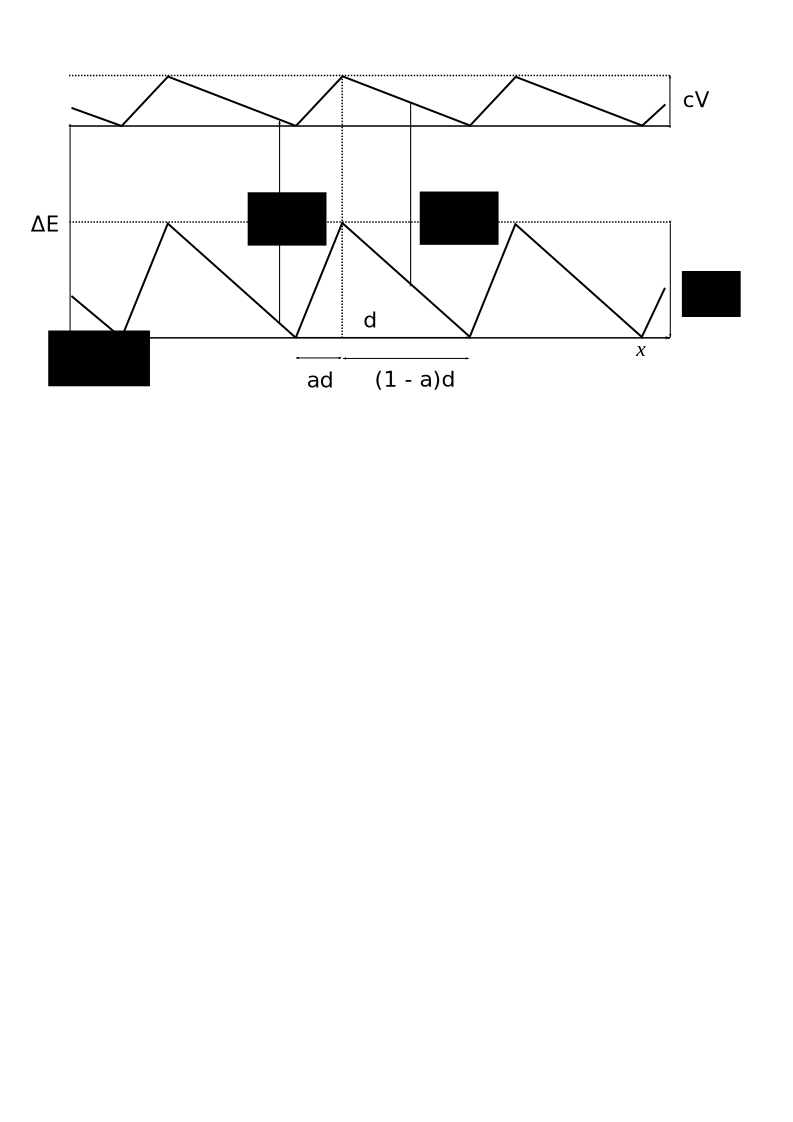
\includegraphics[width=0.45\textwidth,height=!]{energy}
\caption{Energy landscape in which the myosin motor diffuses, relative to the actin filament.}
\label{Fig: energy}
\end{figure}
 We can measure and average these quantities in our simulations and we can define a chemical efficiency as follows
\begin{equation}
\eta = \frac{\langle\mathcal Q_{in}\rangle+\langle\mathcal Q_{out}\rangle}{\langle\mathcal Q_{in}\rangle} .
\label{eq:efficiency}
\end{equation}
This quantifies the fraction of chemical energy, supplied by the ATP driven cycles of the heads, that remains in the system. 
This is shown in figure \ref{Fig: chem}.
\begin{figure}[b]
\centering
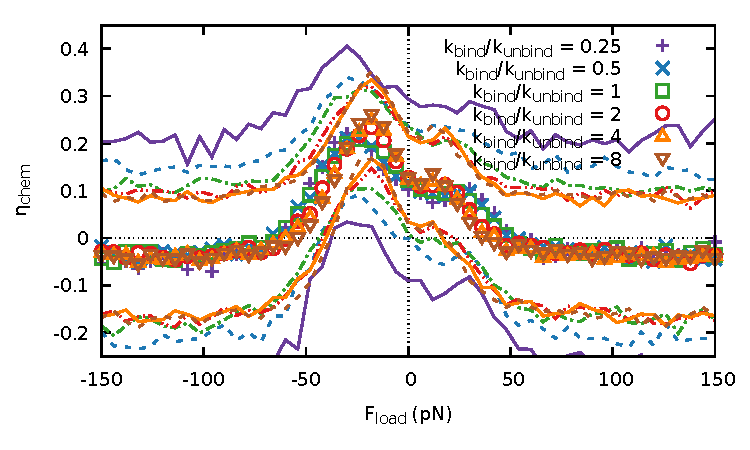
\includegraphics[width=0.45\textwidth,height=!]{chemical_cycle}
\caption{Chemical efficiency $\eta$ as a function of load force $F_\text{load}$.
By increasing the $k_d/k_a$ ratio the local maximums of chemical efficiencies are getting closer origin,
and their fluctuations decrease. 
}
\label{Fig: chem}
\end{figure}


After each jump in the chemical state of a motor head, the potential in which the whole motor diffuses is altered and a new relaxation process takes place. 
The relaxation times of these diffusion processes are much faster than the times between chemical jumps. 
This is because the chemical rates of the motor heads are very small. 
Hence we can assume that the means of the quantities (\ref{q_in}) and (\ref{q_out}) can be described by
\begin{gather}
\begin{aligned}[b]
\langle \mathcal Q_{in} \rangle 
=& \rho^{eq}_1 k_d \left[ \Delta E - (1-c)\langle V_r(x) \rangle_{s=1} \right] \\
=& \frac{k_a k_d}{k_a + k_d}\left[\Delta E - (1-c)\langle V_r(x) \rangle_{s=1} \right] 
\end{aligned}
\label{Q_in} \\
\begin{aligned}[b]
\langle \mathcal Q_{out} \rangle 
=& -\rho^{eq}_0 k_a \left[ \Delta E - (1-c)\langle V_r(x) \rangle_{s=0} \right] \\
=& -\frac{k_a k_d}{k_a + k_d} \left[ \Delta E - (1-c)\langle V_r(x) \rangle_{s=0} \right] 
\end{aligned}
\label{Q_out}
\end{gather}
where $\langle \cdot \rangle_{s}$ stands for an average over the steady state distribution in a given state $s$. 
This will give us an expression for the chemical efficiency.
\begin{equation}
\eta = \frac{ (1-c) \left( \langle V_r \rangle_{s=0} - \langle V_r \rangle_{s=1} \right) }{ \Delta E - (1-c) \langle V_r \rangle_{s=1} } \label{eta}
\end{equation}
From this, we can understand the chemical energy balance, shown in figure \ref{Fig: chem}, by looking at the difference of where a motor head is typically positioned in the potential energy landscape when it is in the attached or detached state. 
These distributions are computed by collecting the positions of the heads over all times that the head was in the attached/detached state. 
They are shown in figure \ref{Fig: pos_distr} for different load forces. 
As argued, since the relaxation is fast, compared to the chemical rates, this approximates the steady distribution very well.
\begin{figure*}[t]
\centering
\subfigure[Attachable state]{ 
\centering
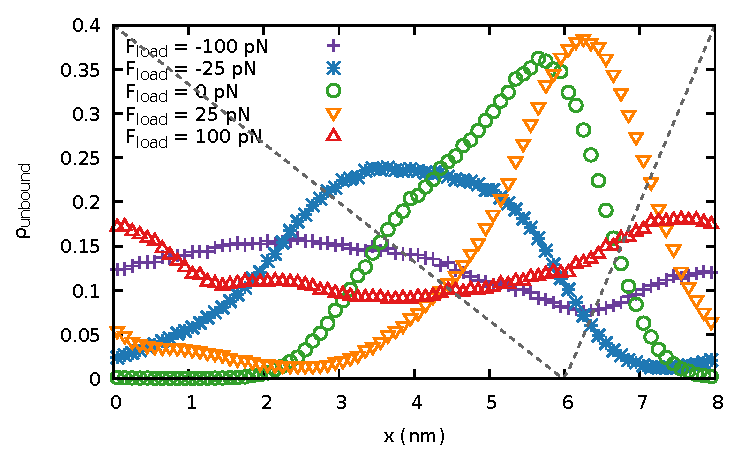
\includegraphics[width=.45\textwidth,height=!]{pos_distr_a_F}
}
\subfigure[Detached state]{
\centering
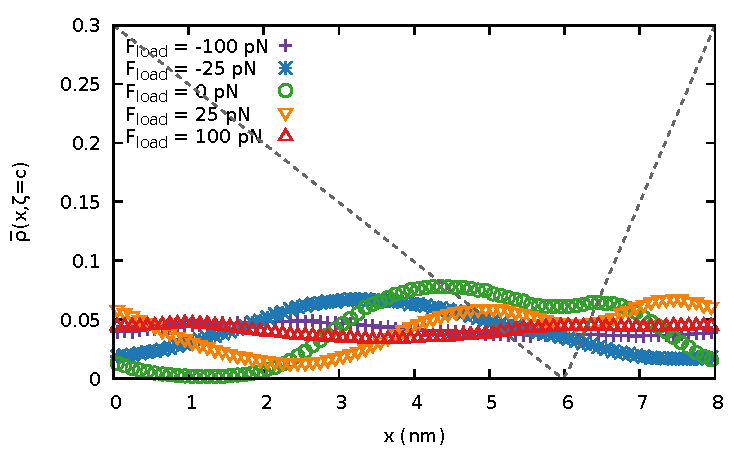
\includegraphics[width=.45\textwidth,height=!]{pos_distr_d_F}
}
\caption{Spatial distributions $\rho$ of individual heads of the motor with respect to the ratchet potential (denoted by dashed black line) for different load forces $F_\text{load}$.
The spatial distribution is taken as the average over all heads at the given motor in a given internal state.
We observe that heads in the attachable state follow the potential closely while those in the detached state do not. 
Also by increasing the external load, all distributions universally become flat. 
}
\label{Fig: pos_distr}
\end{figure*}
In the case without an external load, $F_{load}=0$, the motor head is very unlikely to cross the potential barrier in the attached state. 
The maximum of the distribution is close to the minimum of the potential. 
The discrepancy comes from the fact that the motor has multiple head with a fixed distance between them, which does not match with the period of the ratchet potential. 
Also the fact that the distributions seem to exhibit multiple peaks, can be attributed to the motor having four heads. 
Both in the attached and detached state, the head can be found predominantly on the soft slope of the ratchet, which is to be expected.


With increasing load, we see both a shift of the maximum and a flattening of the profile. 
The detached distributions are broader for $F_{load}=0$, because to potential is lower and less steep, and also seem to be more susceptible to external forces, i.e. the profile gets more. 


To understand the dependency of the chemical efficiency on the load, we must compare the attached and detached distribution and correlate this with the with of the energy gap along the period of the ratchet. 
After all, the numerator in $\eta$ is proportional to $\Delta E - V(x) \left[ \rho_a(x) - \rho_d(x) \right]$ integrated over a period of the ratchet. 
This quantity is plotted in figure \ref{Fig: chem_energy_distr}
\begin{figure}[b]
\centering
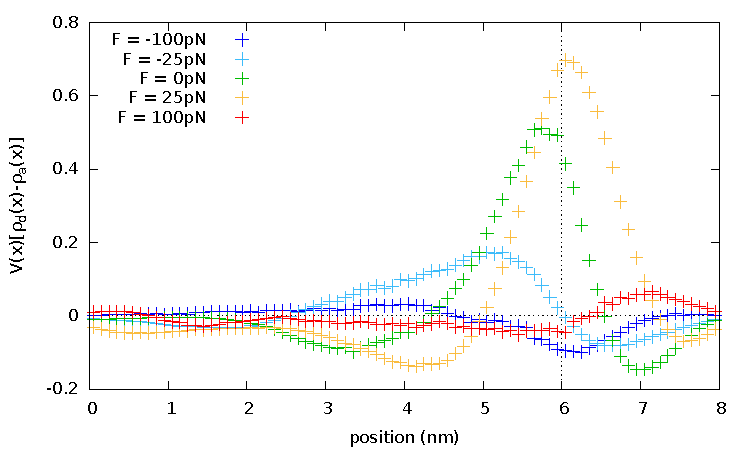
\includegraphics[width=0.45\textwidth,height=!]{chem_energy_distr_all_F}
\caption{Density of the nett energy output \eqref{} produced by the chemical cycle for various load forces $F_\text{load}$. %TODO
We observe that the optimal output is achieved when there is the biggest discrepancy between spatial distributions, see figure~\ref{Fig: pos_distr}. 
}
\label{Fig: chem_energy_distr}
\end{figure}


For example, in absence of a load, the distribution in the attached state is peak around the potential's minimum and has a higher amplitude there compared to the distribution in the detached state. 
In this region, the energy gap is larger than around the maximum of the potential. 
Therefore more energy goes into the system, when ATP binds to a head, than energy going out, when ATP is hydrolyzed and the head attaches again to the actin filament. 


When the load is increased to $F_{load} = 25 \, \mathrm{pN}$, the distributions shift to the right but distribution for the attached state remains peaked around the potential minimum, while the detached distribution flattens out and increases around the potential maximum. 
This leads to an increase of $\eta$. 
For a load in the opposite direction $F_{load}= -25 \, \mathrm{pN}$ the effect on $\eta$ is similar but less pronounced, since the slope of the ratchet on the side is less steep and the distributions get more spread out. 


For larger loads, the distributions shift more but since the detached one is flatter, it is more plausible the find a head in the detached state around the potential minimum. 
This means that more energy will be dissipated when the heads bind and $\eta$ will go down and even become negative. 
In the next section we will investigate the behavior of $\eta$ for large loads and show that it indeed has to be negative and that it will decay like $\frac{1}{F_{load}^2}$ as $F_{load}$ goes to infinity.

\section{Perturbative treatment}
In this section we will show that the chemical cycle must extract energy from the ratchet system with one head and for large load forces, i.e. the chemical efficiency $\eta$ must be negative. 
We will do this by calculating the perturbative corrections to the probability density of the position of the motor with respect to the actin filament, both in the attached and detached state. 
For this we assume that the diffusive relaxation time is much shorter than the typical time between jumps in the chemical state of the heads. 
This will allow us to use steady state distributions to calculate the expected values of the potential energy in equation (\ref{eta}).
We start with the Fokker-Planck equation for steady states, i.e. $\partial_t \rho = 0$.
\begin{equation}
\frac{1}{\gamma} \partial_x \left[ \left( F - \partial_x V_r(x) \right) \rho(x) - k_B T \partial_x \rho(x) \right] = 0
\label{FP_ss}
\end{equation}
where $V$ is the ratchet potential in a given state and F is the constant load force. 
As we want to calculate perturbations for large loads we will rewrite equation (\ref{FP_ss}) so that we can use $\epsilon = \frac{1}{F}$ as the perturbation.
\begin{equation}
\partial_x \left[ \rho(x) - \frac{1}{F} \left( \partial_x V_r(x) \rho(x) + k_B T \partial_x \rho(x) \right) \right] = 0
\label{FP_ss_pert}
\end{equation}
For infinitely large loads the steady state distribution is flat, i.e. $\rho_0 = \frac{1}{d}$, which will be the zeroth order solution. 
Since this will be the case in both the attached and detached state, it will yield the same expected values of $V$ and therefore $\eta$ must be equal to zero.
The first order solution will be of the form $\rho_1 = \rho_0 + \delta\rho_1$. 
When inserted into (\ref{FP_ss_pert}) and only keeping terms up to first order in $\frac{1}{F}$, we get
\begin{equation*}
\partial_x \left[ \delta \rho_1 - \frac{1}{F} \partial_x V_r(x) \rho_0 \right] = 0
\end{equation*}
or alternatively
\begin{equation*}
\delta\rho_1 = \frac{1}{dF} \partial_x V_r + C
\end{equation*}
where $C$ is an integration constant that, after normalization of $\rho_1$, must be equal to $0$.
However, this first order correction will not contribute to calculations of $\langle V_r \rangle_\rho$ since
\begin{align*}
\langle V_r \rangle_{\delta\rho_1} 
&= \int_0^d V_r(x) \, \delta\rho_1 \; \rmd x
\propto \int_0^d V_r(x) \, \partial_x V_r(x) \; \rmd x \\
&= \frac{1}{2} \int_0^d \partial_x V_r^2(x) \; \rmd x 
= 0
\end{align*}
where we used integration by parts and the fact that $V_r(x)$ is periodic.
Consequently, we need to calculate the second order correction $\delta\rho_2$. 
Now by inserting $\rho_2 = \rho_1 + \delta\rho_2$ in (\ref{FP_ss_pert}) and only keeping up to second order in $\frac{1}{F}$, we find
\begin{multline*}
\partial_x \left[ \delta\rho_2 - \frac{1}{F} \partial_x V_r \, \delta\rho_1 - \frac{k_B T}{F} \partial_x \delta\rho_1 \right] \\
= \partial_x \left[ \delta\rho_2 - \frac{1}{ d F^2 } \left(\partial_x V_r\right)^2 - \frac{k_B T}{dF^2} \partial_x^2 V_r \right] 
= 0
\end{multline*}
which solves to
\begin{equation*}
\delta\rho_2 = \frac{1}{ d F^2} \left[ \left( \partial_x V_r \right)^2 - k_B T \partial_x^2 V_r \right] + C^\prime.
\end{equation*}
Again by normalization, the integration constant $C^\prime$ can be determined.
\begin{multline*}
1 = \int_0^d \rho_2 \; \rmd x 
= \int_0^d \left\{ \frac{1}{d} + \frac{1}{ d F } \partial_x V_r \right\} \; \rmd x \\
+ \int_0^d \left\{  \frac{1}{ d F^2 } \left[ \left( \partial_x V_r \right)^2 - k_B T \partial_x^2 V_r \right] + C^\prime\right\} \; \rmd x 
\end{multline*}
Which simplifies to
\begin{equation}
C^\prime = - \frac{1}{ d^2 F^2 } \int_0^d \left( \partial_x V_r \right)^2 \; \rmd x . 
\end{equation}
The first order term again did not contribute and the thermal term vanished as well because of the periodicity of $V_r(x)$. 
Now the density up to second order is given by
\begin{align*}
\rho_2 =& \rho_0 + \delta\rho_1 + \delta\rho_2 \\
=& \frac{1}{d} + \frac{1}{d F} \partial_x V_r +{} \\
&+ \frac{1}{d F^2} \left[ \left( \partial_x V_r \right)^2 - k_B T \partial_x^2V_r - \frac{1}{d} \int_0^d \left( \partial_x V_r \right)^2 \; \rmd x \right] .
\end{align*}
Observe that in this form, the depends on the ratchet potential only through a first or second order derivative. 
Therefore the density will appear as a piecewise constant function on $x\in[0,l]$, with different values for $x < a l$ and $x > a l $. 
This trend can already be seen in the empirical density obtained from simulations for large load forces $F_L = \pm 250 \, \mathrm{pN}$ in figure %TODO
\begin{figure*}[t]
\centering
\subfigure[Positive load]{
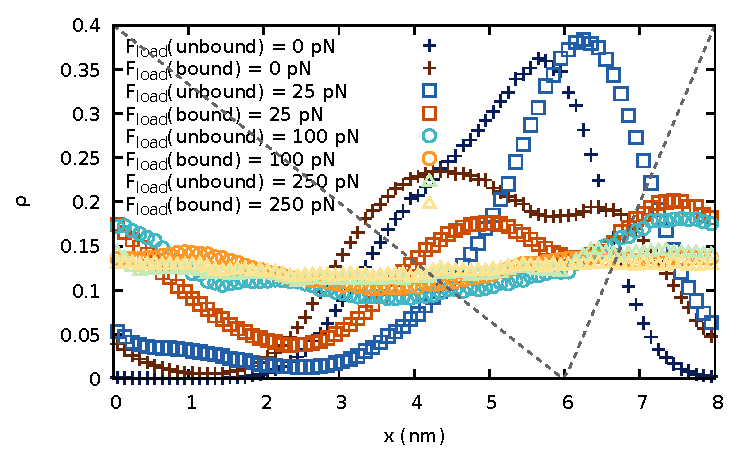
\includegraphics[width=0.45\textwidth,height=!]{pos_multiplot_p}
}
\subfigure[Negative load]{
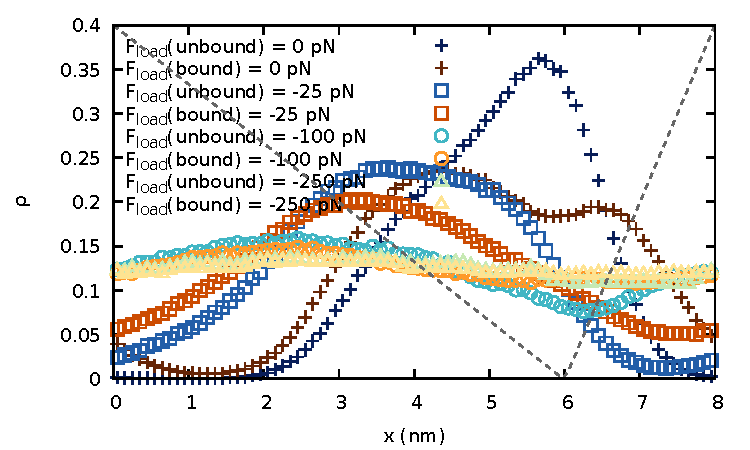
\includegraphics[width=0.45\textwidth,height=!]{pos_multiplot_m}
}
\caption{Side by side comparison of empirical density profiles in both attachable (a - blue colored) and detached (d - red colored) state for different loads.
Profiles sharing the same load magnitude $|F_\text{load}|$ are denoted by the symbols.
}
\label{Fig: pos_multiplot}
\end{figure*}


With the second order correction we can now calculate the expected value of the potential energy.
\begin{align*}
\langle V_r \rangle_{\delta\rho_2} 
=& \int_0^d V_r(x) \, \delta\rho_2 \; \rmd x \\
=& \frac{1}{d F^2} \int_0^d V_r(x) \left(\partial_x V_r \right)^2 \; \rmd x  \\
&- \frac{1}{d^2 F^2} \int_0^d V_r(x) \; \rmd x \int_0^d \left( \partial_y V_r \right)^2 \; \rmd y \\
&- \frac{k_B T}{d F^2} \int_0^d V_r(x) \, \partial_x^2 V_r \; \rmd x
\end{align*}
The first two terms will cancel each other and after carrying out the integral for the third term, with $V_r(x)$ given by (\ref{rat_pot}), one finds 
\begin{equation}
\langle V_r \rangle_{ \delta\rho_2, s=1} = \frac{k_B T}{F^2} \frac{V^2}{a \left(1-a\right) d^2 }
\end{equation}
For the expectation value in the detached state, the potentials appearing in the expression for the distributions must be rescaled by a factor $c$, which leads to
\begin{equation}
\langle V_r \rangle_{\delta\rho_2, s=0} = \frac{k_B T}{F^2} \frac{c V^2}{a \left(1-a\right) d^2 } .
\end{equation}
Similarly, for the zeroth order expectation value we find
\begin{equation}
\langle V_r \rangle_{\rho_0} = \frac{1}{d} \int_0^d V_r(x) \; \rmd x = \frac{V}{2} .
\end{equation}
Using this, we can calculate $\eta$ up to second order in $\frac{1}{F}$. 
Note that the zeroth and first order are zero.
\begin{equation}
\eta = -\left( \frac{V}{d F} \right)^2 \frac{k_B T} { \Delta E - (1-c) \frac{V}{2} } \; \frac{ \left(1-c\right)^2 }{ a (1-a) }
\end{equation}
With this we show that, at least for a ratchet system with one motor head, it is expected that $\eta$ will become negative for large external loads and eventually goes to zero as the load goes to infinity. 
This means the driven system looses chemical energy, while the external force is performing work on the system. 
The efficiency $\eta$ is symmetric in $F$ for large forces, which is also apparent from figure \ref{Fig: chem}. 
Also note that in the expression for the chemical efficiency, the ratio between the amplitude of the ratchet potential $V$ and the work done by the external force over a period of the potential $d F$ appears in the formula, as well as the ratio between the thermal energy $k_B T$ and the mean energy gap between the attached and detached state. 
Indeed for large load on the motor, the efficiency will go to zero as can be seen from the zeroth order solution.
\par
In addition we can compute the current using the obtained densities. 
The current is taken from the Fokker-Planck equation (\ref{FP_ss}).
\begin{equation}
\mathcal{J} = \frac{1}{\gamma} \left[ \left( F - \partial_x V_r \right) \rho - k_B T \partial_x \rho \right] 
\end{equation}
When inserting $\rho_2$, we find the current in leading orders of $F$.
\begin{align*}
\mathcal{J} =& \frac{F}{\gamma d} \left( 1 + C^\prime \right) + \mathcal{O}( \frac{1}{F^2} ) \\
=& \frac{F}{\gamma d} - \frac{1}{F\gamma d^2} \int^d_0 \left( \partial_x V_r \right)^2 \; \rmd x + \mathcal{O}(\frac{1}{F^2}) 
\end{align*}
Important to note is that the current, integrated over the period of the ratchet, represents the mean velocity of the motor. 
Indeed, the dominant term for large external forces is $\mathcal{J}_0 = \frac{F}{\gamma}$, which was also apparent from the simulations shown in figure \ref{Fig: F_v}. 
Furthermore, the force-independent term vanishes leading to an anti-symmetric form with respect to $F$. 
The first correction is given by $\frac{F}{\gamma}C^\prime\propto \frac{1}{F}$. 
This decay was clearly seen in figure \ref{Fig: eff_frict_decay}, which depicts was the mean motor velocity deduced by the drag velocity due to the load force $\frac{F}{\gamma}$. 
This isolates the contribution from the ratchet potential. 
Hence this result, obtained for a one-headed motor, also seems to hold for the simulations of motors with four heads. 

In fact, if we compare the chemical efficiencies for a motor with one head and four heads, we see a great similarity.
This comparison is made in figure \ref{Fig: chem_eff_1head}.
\begin{figure}[t]
\centering
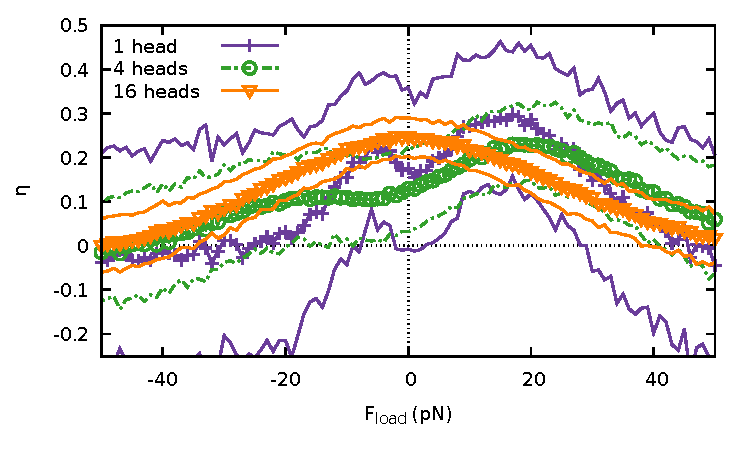
\includegraphics[width=0.45\textwidth,height=!]{chemical_cycle_1head}
\caption{Chemical efficiency of a motor under load. 
Comparison of one (red triangles), four (blue stars), sixteen (green circles) headed motors.
We observe that with increasing number of heads the efficiency \eqref{eq:efficiency} distribution 
gets broader and it's variance decreases.
Moreover, for sixteen heads it became centered without two local maximas. 
}
\label{Fig: chem_eff_1head}
\end{figure}
The behavior for large load forces seems to be exactly the same.
Since $\eta$ is a ratio of chemical energies exchanged through the motor heads, this means that for large enough forces a head of the four headed motor no longer feels the presence of the other heads.
However the one headed motor is more susceptible to external forces as it's chemical efficiency starts to drop already at smaller loads. 
Note that the curves with higher detach rate $k_d$ in figure \ref{Fig: chem} tend to approach the curve for one head in figure \ref{Fig: chem_eff_1head}. 
When the detach rate is increased, the configuration where fewer heads of the motor are attach to the polymer indeed becomes more likely.


Another trait of the chemical efficiency curves are the local minima's around $F_{load}=0$. 
The understand this we must again look at equation (\ref{eta}) which is determined by the ratchet potential averaged with the heads' distribution in the attached and detached state. 
For a one headed motor, these distribution will both be peaked around the minimum of the ratchet potential. 
In fact, the distributions will be given by the Boltzmann distribution.
\begin{equation}
\rho_s (x) = e^{-\beta \zeta(s) V_r(x)}
\end{equation} 
From this point of view, detaching the head is equivalent to an increasing of the temperature $T\rightarrow\frac{T}{c}$. 
Hence the distributions for the detached state are broader and the expectation value of $V_r$ will be bigger than in the attached state and $\eta$ will be positive. 
Now if we apply a small external force, the distributions will be slightly perturbed and given by the McLennan formula
\begin{equation}
\rho_s^*(x) \propto e^{-\beta \left[V_r(x) - F x\right]}\propto \rho_s(x)\left[1 + \beta F x\right]
\end{equation}
which will, for small $F$, lead to a shift of the distribution $\rho_s$ along the $x$-axis and in the direction of the load. 
In the detached state this will cause a larger displacement than in the attached state because of the potential in that case is less steep. 
A larger displacement of the distribution, away from the potential's minimum, means that $\langle V_r \rangle_{s=0}$ will increase more than $\langle V_r \rangle_{s=1}$ and hence $\eta$ has to increase. 
For a four headed motor, the distributions of the heads at zero load are not exactly peaked around the minimum of the potential because of the fixed distance between each head,  which does not correspond to the period of the ratchet. 
Therefore the local minimum of $\eta$ lies not exactly at, but close to, $F_{load} =0$.
This argument can be further supported by Jensen's inequality, which follow from the fact the the ratchet potential is convex. For this case the inequality reads as follows.
\begin{equation}
V_r(\langle x \rangle) \leq \langle V_r(x) \rangle
\end{equation} 
A lower bound on the expectation value of $V_r$ is given by the value of $V_r$ at the mean position of the heads in a given state. 
In the detached state this position will be farther away from the minimum of the ratchet so the lower bound is higher than in the attached case.

\section{Tug of war}
In  section III we saw that the motor offers resistance when pulled by an external force. 
Now we will look at the motor in a setup where it is subjected to different stiffnesses of the environment in which the filaments are able to move. 
This setup is sketched in figure \ref{Fig: tug}. 
\begin{figure}[t]
\centering
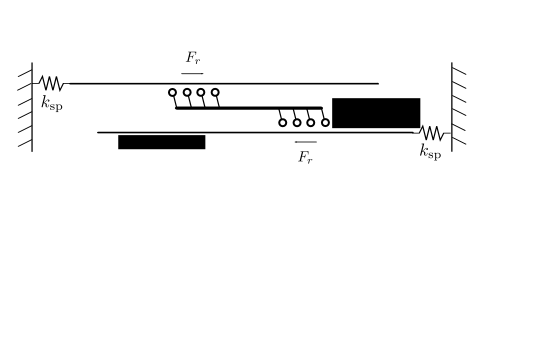
\includegraphics[width=0.45\textwidth,height=!]{tug}
\caption{Illustration of a motor pulling on two actin filament that are each connect to a wall by a spring.}
\label{Fig: tug}
\end{figure}
One can imagine the filaments being part of a large network that is characterized by an elastic constant $k$. 
The motor is now interacting with two filament that are arranged in an anti-parallel fashion. 
Hence it will no longer have a preferred direction to move in and its mean velocity will be zero. 
The observable of interest is now the mean force that the motor applies on the filaments, which is measured through the extension of the springs attached to the filaments. 
This quantity is plotted in figure \ref{Fig: tug_k} for different stiffnesses $k$ of the surrounding network.
\begin{figure}[t]
\centering
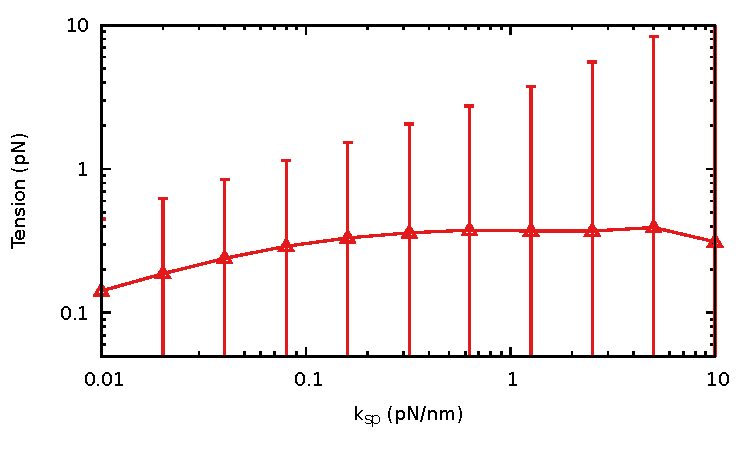
\includegraphics[width=0.45\textwidth,height=!]{tug_k}
\caption{Mean force $F_\text{fil}$ generated by the motor on one of the filaments for varying spring stiffness $k_\text{sp}$.
Lower stiffness enables the polymers to find a local minimum of the ratchet potential more easily, 
thus the exerted force is lower as the contribution of ratchet potential is minimized. 
On the other hand, high stiffness leads to saturation of the exerted force as the main contribution is given by ratchet potential. 
}
\label{Fig: tug_k}
\end{figure}
The force with which the motor pulls on the filament depends strongly on this elasticity $k$ and saturates for large $k$. 
This suggests that the motor is able to sense its environment's mechanical properties.
Similar results were obtained for different motor models with load dependent chemical rates \cite{stam2015isoforms,albert2014stochastic}.
Here we show that the simple ratchet model with constant rates already captures the characteristic. However it is important to include the large fluctuations in this model to preserve the mechanosensing behavior. In some models the force-velocity relation is implemented ad-hoc, such that the velocity of the motor is deterministic and it depends only on the load. In those models the motor will essentially stall in this setup and 
cease to pull on the filaments. Therefore mechanosensing will not occur spontaneously in those models.

\section{Tug of war II}

Filaments connected to beads with spring. 
Pull beads with constant velocity.
\begin{figure}[t]
\centering
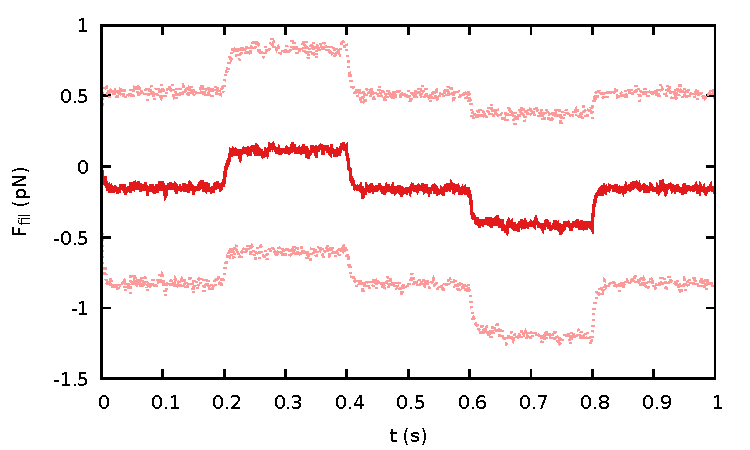
\includegraphics[width=0.45\textwidth,height=!]{tug_v}
\caption{Mean force $F_\text{fil}$ exerted by the motor on one of the filaments during a stretch-compression cycle of the beads.}
\label{Fig: tug_v}
\end{figure}
Look into: Work done during cycle.
\section{Tug of war III}

No springs but constant load on both filaments.\newline
Force-velocity relation.\newline
\begin{figure}[t]
\centering
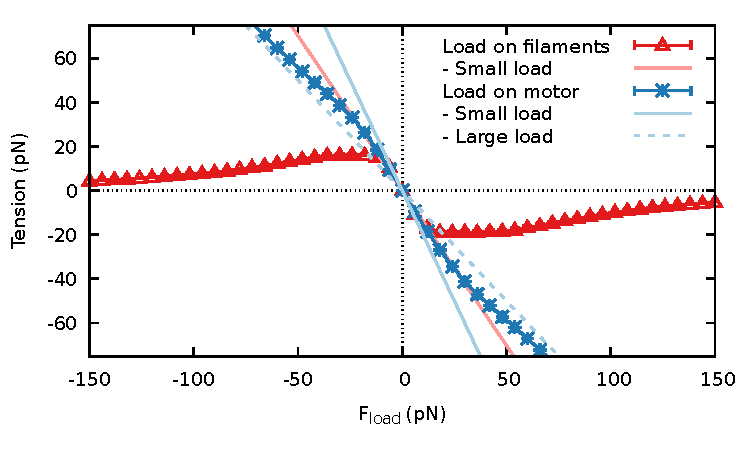
\includegraphics[width=0.45\textwidth,height=!]{tug_F}
\caption{Analogue to figure~\ref{Fig: effective_force}, now with 2 filaments instead of 1.}
\label{Fig: tug_F}
\end{figure}
Movement of motor.
\begin{figure}[t]
\centering
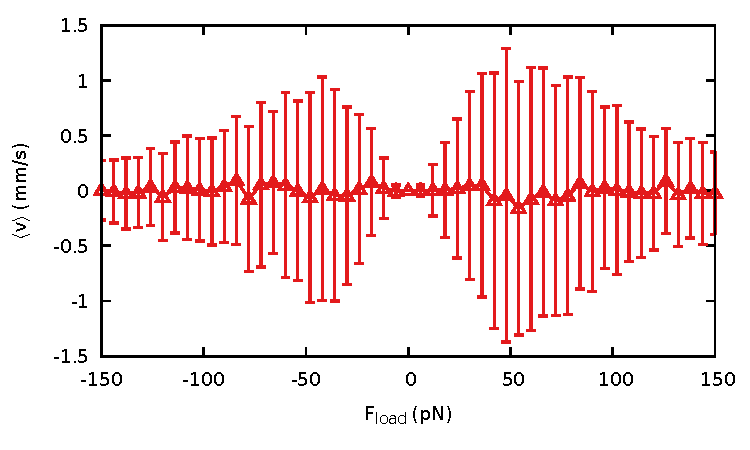
\includegraphics[width=0.45\textwidth,height=!]{tug_F_motor}
\caption{Displacement of frustrated motor in between the filaments.} %TODO
\label{Fig: tug_F_motor}
\end{figure}

\newpage
\section{TO DO}
\begin{itemize}
\item Extra data for some plots
\item Simulation data for $1/F^2$ tail of $\eta$
\item Explicitly plot result for second order distribution against empirical result
\item Tug of war section
\item Intro
\item References
\end{itemize}


\bibliography{ratchet}


\end{document}
